\chapter{Inledning}

Mängden av producerad data ökar helta tiden, och kräver därför kraftigare och pålitligare
metoder för att hantera datan. Ett exempel på helheter som skapar mycket data i form av
dataströmmar är sakernas internet (Internet of Things, IoT) system som smarta städer
(eng. Smart Cities) var data amlas från sensorer och mobiltelefoner \citep{vakali2014smart}
eller i sjöfart var data samlas från skepp \citep{xu2019internet}. Utvinnande och analysering
av massiva dataströmmar har blivit mera aktuellt eftersom nätverksinfrastrukturen förbättras.

Inkommande datan är kan oftast inte direkt sparas eller analyseras. Därför är det normalt att
segmentera, filtrera eller grupera datan före själva analyseringen utförs på datan.
Datan kan också komma från många olika källor \citep{beringer2006online} som kräver sammanslagning
av datan från källorna. Eftersom mängden data och behovet för analysering av realtids data växer
är behovet för komplexare arkitekturer för databehandling större. Denna texten fokuserar på metoder för
bearbetning av massiva dataströmmar på arkitekturnivå. Vi går även 
igenom några platformer som används för distribuerad bearbetning av dataströmmar.

Det finns två olika sätt för behandling av dataströmmar: Lambda arkitektur 
($\lambda$-arkitektur) och Kappa arkitektur ($\kappa$-arkitektur). Det visar sig att
båda akitekturerna har nackdelar, och att beroende på vilken man väljer måste man
offra performans eller komplexitet \citep{mci/Feick2018}.

Avhandlingen beskriver och jämför både $\lambda$ och $\kappa$ arkitekturen. Bakgrundskunskaperna
för båda arkitekturerna introduceras i kapitel 2 och kapitel 3 går 
igenom några platformer för distribuerad bearbetning. I kapitel 5 diskuteras tilfällen var $\kappa$ 
eller $\lambda$ arkitektur kan användas.

\section{Använda betäckningar}

I texten används olika betäckningar för att beskriva datastrukturer och deras operationer. Betäckningarna är beskrivna i tabellen nedan.

\begin{tabular}{ |p{3cm}||p{8cm}|  }
 \hline
 \multicolumn{2}{|c|}{Betäckningar} \\
 \hline
 Betäckning & Beskrivning\\
 \hline
  $A$[]   &  En lista med element av typ A \\
 $S$[$a$]   &  Läsoperationen av en lista eller dataström $S$. $a$ är indexet för läsoperationen \\
 $(A, B)$   &  En tupel var vänstra värdet är av typ A och högra värdet är av typ B\\
 $S$ & Teckensekvens (eng. string)\\
 \hline
\end{tabular}



\chapter{Introduktion}

Detta kapitel går igenom gruderna för dataströmmar och olika behandligsmetoder. Kapitlet antar att
läsaren kan grunderna i programmering, algoritmer, datanätverk och matematik på kandidatnivå i datavetenskap.

\section{Dataströmmar}

En dataström kan tänkas vara en lista $S$ med $n$ element. Elementen kans läsas från listan med operationen $S$[$t$] 
var $t$ är tidsstämpeln av nutiden. Värden kan inte läsas med framtida eller förflutna tidsstämplar. Listan läses
så ofta som möjligt och evetuella värden behandlas sedan. Eftersom datan är i form av en ström kan vissa 
tidsstämplar ge odefinierade värden, som ignoreras.

\begin{verbatim}
    while (value = stream.readNext()) {
      if (isDefined(value)) {
        processStreamValue(value)
      }
    }
\end{verbatim}

Datan från dataströmmar kan levereras på många olika sätt. Inom IoT är det normalt att dataströmmar 
levereras över TCP/IP \citep{shang2016challenges}. Dataströmmen kan till exempel behandlas med mjukvara som körs på en server eller ett kluster av många servrar.

Bild, mera källor, bättre matematisk beskrivning?

\section{Intagning av dataströmmar}

Intagning (eng. ingestion) av dataströmmar är prosessen var datan hämtas eller mottags från en extern källa.
En platform som används ofta för intagning av data Apache Kafka. Kafka är en platform som fungerar med
en producent/konsument modell (eng. producer/consumer model) [Kafka]. I praktiken betyder det att inkommande data läses av konsumenter och produceras av producenter [Fig1].

\begin{figure}[h]
    \centering
    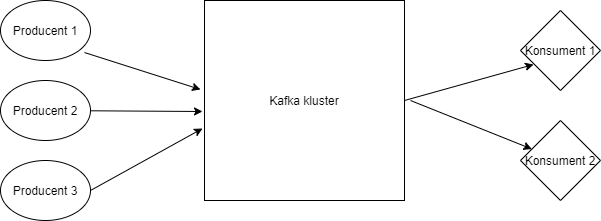
\includegraphics[scale=0.7]{src/thesis/img/prod-cons-model.png}
    \caption{Producent/konsument modellen med ett Kafka kluster.}
    \label{fig:mesh1}
\end{figure}

Datan som produceras av producenter i Kafka är händelser (eng. events). Händelserna har 3 olika
element: ett nyckelvärde, själva värdet av händelsen och en tidsstämpel. Till exempel, om vi har ett Kafka kluster som intar telemetri från fartyg på havet så kan nyckelvärdet vara ett unikt nummer som fartyget har i ett datasystem så att händelsen kan kopplas samaan med information av fartyget, värdet är kursen av fartyget och tidsstämpeln tiden när fartyget har skickat händelsen.

Kafka ger också möjligheten att dela in händelser i olika kategorier tom kallas ämnen (eng. topics). Konsumenterna prenumererar till olika ämnen och får händelser från prenumererade ämnen.

\section{MapReduce}

När vi har förmågan att inta data från en dataström behöver vi också ett sätt för att hantera, slå ihop och analysera datan som kommer in. En mycket använd model är MapReduce modellen. MapReduce är en programmeringsmodel som kan bearbeta massiva mängder data på ett kluster av datorer \citep{dean2008mapreduce}. MapReduce baserar sig på två funktioner 
som är bekanta från funktionella programmerings paradigmen, \textit{map} och \textit{reduce}. Data splittras först i mindre bitar och bitarna ges till MapReduce \textit{arbetare} (workers) som körs på en annan maskin eller process från huvudprocessen. Varje arbetare
kan få en eller flera bitar av datan. Arbetarna kör först funktionen map på datan och sedan reduce.

\subsection{Map och Reduce funktionerna}

MapReduce modellens map funktion kan beskrivas som en funktion $f: A \rightarrow B$ var $A = (S, S)$ och $B = (S, K)$ var $K$ är typen av datan som returneras. Map funktionen kan användas för till exemple filtrering,
transformering eller tolkning av serialiserad data. Funktionen returnerar en lista av tuplar som innehåller nyckeln och värdet. Map funktionen kans se ut till exempel såhär:

\begin{verbatim}
    def map(key: S, persons: S[]): (S, S)[] = {
      groupedByNameLength = persons.groupByNameLength()
      result = []
      for len in groupedByNameLength:
        append (len, 1) to result
      return result
    }
\end{verbatim}

MapReduce modellens reduce funktion tar in datan som returneras från map funktionen och slår ihop datan. 

\begin{verbatim}
    def reduce(keyFromMap: S, valueFromMap: (Int, Int)[]): Integer = {
      result = 0
      for value in valueFromMap:
        result = result + value
      return result
    }
\end{verbatim}

\subsection{MapReduce processen}

Ett MapReduce program har 7 olika steg. Först splittrats inkommande datan till $N$ segment. Efter splittringen
görs det flera nodar av MapReduce programmet var en nod fungerar som \textit{mästare} (master) och andra
som arbetare. Mästarnoden tilldelar arbetarna map eller reduce arbeten. Arbetarna som har som uppgit att utföra map arbeten
läsen ett segment som mästarnoden har givit den, kör funktionen map och sparar tupel listan i en buffert i minnet.
Innehållet av bufferterna skrivs under jämna mellanrun till en fil och arbetaren signalerar mästarnoden var datan för ett visst
tupel finns i MapReduce klustret. Mästarnoden informerar arbetaren med reduce uppgifter om platser var datan sparad från map skedet
befinner. Datan läses och sorteras sedan så att tuplar med samma nyckel är gruperade tillsammans. Arbetaren kör reduce funktionen på varje
unika nyckel som finns is matade datan. Varje arbetare med ett reduce arbete skriver ut resultatet till en fil.

\begin{figure}[h]
    \centering
    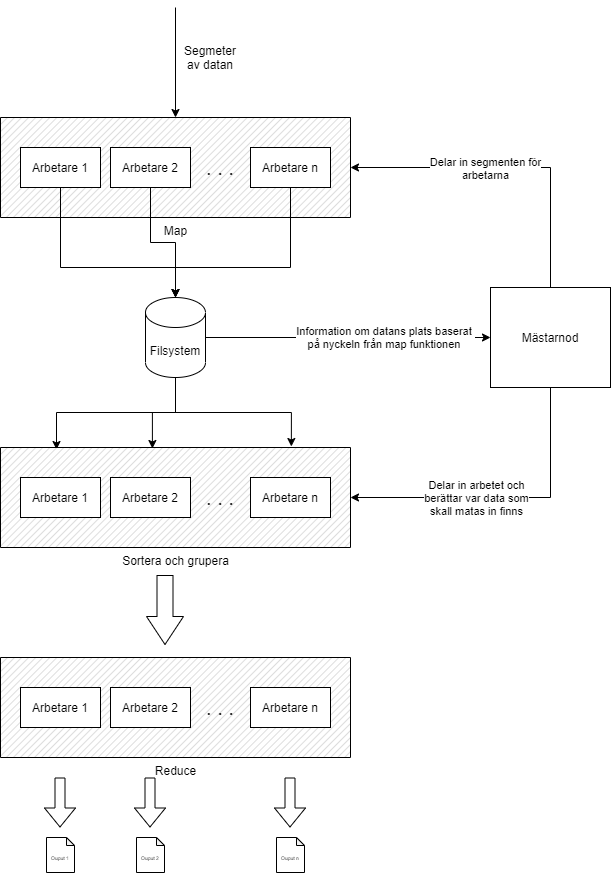
\includegraphics[scale=0.5]{src/thesis/img/map-reduce.png}
    \caption{MapReduce processen}
    \label{fig:mesh1}
\end{figure}

\section{Satsvis bearbetning av dataströmmar}

\textit{Satsvis behandling} (batch processing) av dataströmmar är en metod för behandling av 
dataströmmar som går ut på att köra behandlingsprogram på datan till exempel mellan jämna
tidsinterval eller när någon viss tröskel arr överskridit \citep{marz2013big}. Satsvisa behandligen
innehåller 3 olika steg. I först steget sparas inkommande datan. Inkommande datan kans sparas vart
som hällst, men det är normalt at använda till exemple Apache Hadoops \textit{distribuerade 
filsystem} (Hadoop Distributed File System). I nästa steget processeras datan med till exempel
MapReduce som vi gick igenom i förra kapitlet. MapReduce processens data sparas oftast i en 
nyckel/värde (key-value) databas som sedan kan användas för at servera data tille konsumenter.

\begin{figure}[h]
    \centering
    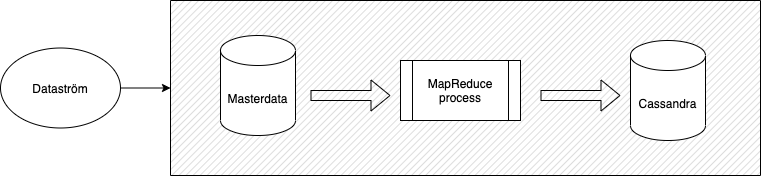
\includegraphics[scale=0.5]{src/thesis/img/batch-pipeline.png}
    \caption{MapReduce processen}
    \label{fig:mesh1}
\end{figure}

\section{Speed behandling}

\chapter{Arkitektur}

\section{Lambda arkitektur}

\section{Kappa arkitektur}

\section{Andra}

\chapter{Sammanfattning}
